\documentclass[11pt, oneside]{article}   	% use "amsart" instead of "article" for AMSLaTeX format


% \usepackage{draftwatermark}
% \SetWatermarkText{Draft}
% \SetWatermarkScale{5}
% \SetWatermarkLightness {0.9} 
% \SetWatermarkColor[rgb]{0.7,0,0}


\usepackage{geometry}                		% See geometry.pdf to learn the layout options. There are lots.
\geometry{letterpaper}                   		% ... or a4paper or a5paper or ... 
%\geometry{landscape}                		% Activate for for rotated page geometry
%\usepackage[parfill]{parskip}    		% Activate to begin paragraphs with an empty line rather than an indent
\usepackage{graphicx}				% Use pdf, png, jpg, or eps� with pdflatex; use eps in DVI mode
								% TeX will automatically convert eps --> pdf in pdflat						
								% TeX will automatically convert eps --> pdf in pdflatex		
\usepackage{amssymb}
\usepackage{mathrsfs}
\usepackage{hyperref}
\usepackage{url}
\usepackage{subcaption}
\usepackage{authblk}
\usepackage{amsmath}
\usepackage{mathtools}
\usepackage{graphicx}
\usepackage[export]{adjustbox}
\usepackage{fixltx2e}
\usepackage{hyperref}
\usepackage{alltt}
\usepackage{color}
\usepackage[utf8]{inputenc}
\usepackage[english]{babel}
\usepackage{float}
\usepackage{bigints}
\usepackage{braket}
\usepackage{siunitx}
\usepackage{adjustbox}
\usepackage{mathtools}
\usepackage{array}
 \usepackage{makecell}
 \usepackage{stackengine}


%
% so you can do e.g., \begin{bmatrix}[r] (or [c] or [l])
%

\makeatletter
\renewcommand*\env@matrix[1][c]{\hskip -\arraycolsep
  \let\@ifnextchar\new@ifnextchar
  \array{*\c@MaxMatrixCols #1}}
\makeatother

\newcommand{\argmax}{\operatornamewithlimits{argmax}}
\newcommand{\argmin}{\operatornamewithlimits{argmin}}


\title{SARS-CoV-2 Spike Protein Cleavage and Fusion}
\author{David Meyer \\ dmm@\{1-4-5.net,uoregon.edu\}}
\date{Last update: \today}							% Activate to display a given date or no date

\begin{document}
\maketitle

\noindent
This sequence of events was described by Jason McLellan TWiV 714 \cite{covid:spike}.

\begin{enumerate}
\item You can get cleavage at S1/S2 site (see Figure \ref{fig:prefusion}) while spike is being produced in the
infected cell since there is	furin present. Here the spike trimer is in the prefusion confirmation.

\item In this case on the surface of an infectous viron the spike protein has already been cleaved at S1/S2. 

\bigskip
\begin{figure} [H]
\center{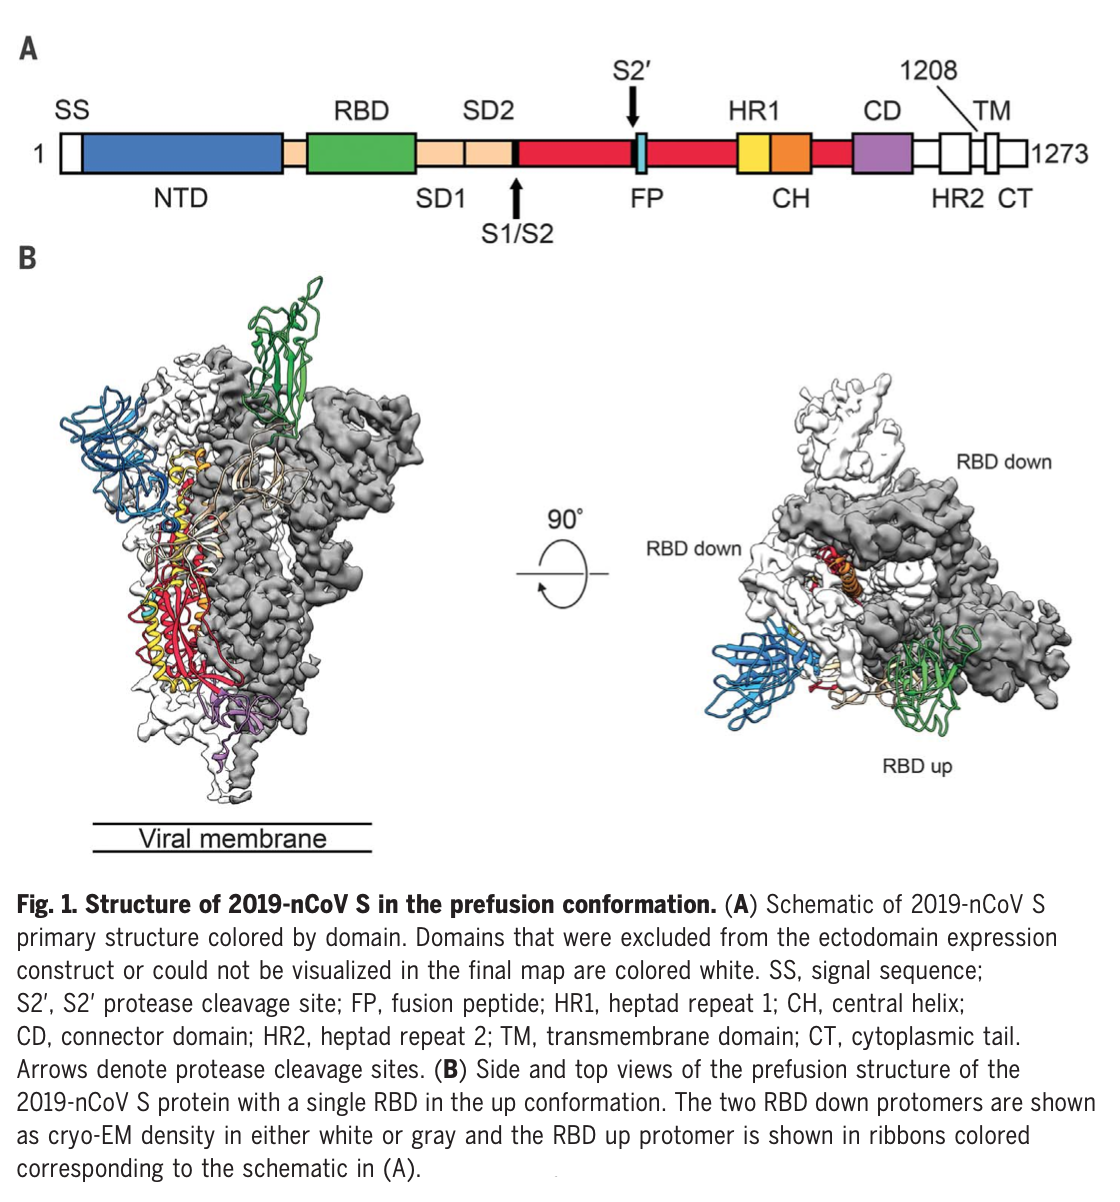
\includegraphics[scale=0.40, frame] {images/prefusion.png}}
\caption{SARS-CoV-2 Spike Prefusion Confirmation \cite{covid:prefusion}}
\label{fig:prefusion}
\end{figure}


\item  Next S1 binds to ACE2 binding at the Receptor Binding Domains (RBDs),
locking one, two or three of the RBDs in the "up" confirmation\footnote{The RBDs are locked 
in the "up" confirmation when bound by ACE2.} which is a thermodynamically unfavorable state.

\item The binding of S1 to ACE2 destabilizes the spike and causes S1 to shed and fall off S2. S1 can be thought of as a "fusion suppressive cap" (like GP120, HA1), which prevents 
the fusion machinery, the spring-loaded S2, from firing.

\item S2 then undergoes a confirmational change and starts rearranging from its spring loaded state, extending
towards the host cell membrane.

\item Cleavage at $\text{S2}^\prime$, usually by TMPRSS2 on the host cell surface or by cathepsin L in an endosome (see Figure \ref{fig:fusion}),  liberates the fusion peptide from the new N-terminal
domain of S2. This allows the S2 now is anchored in the host cell membrane and in the viral membrane.

\bigskip
\begin{figure} [H]
\center{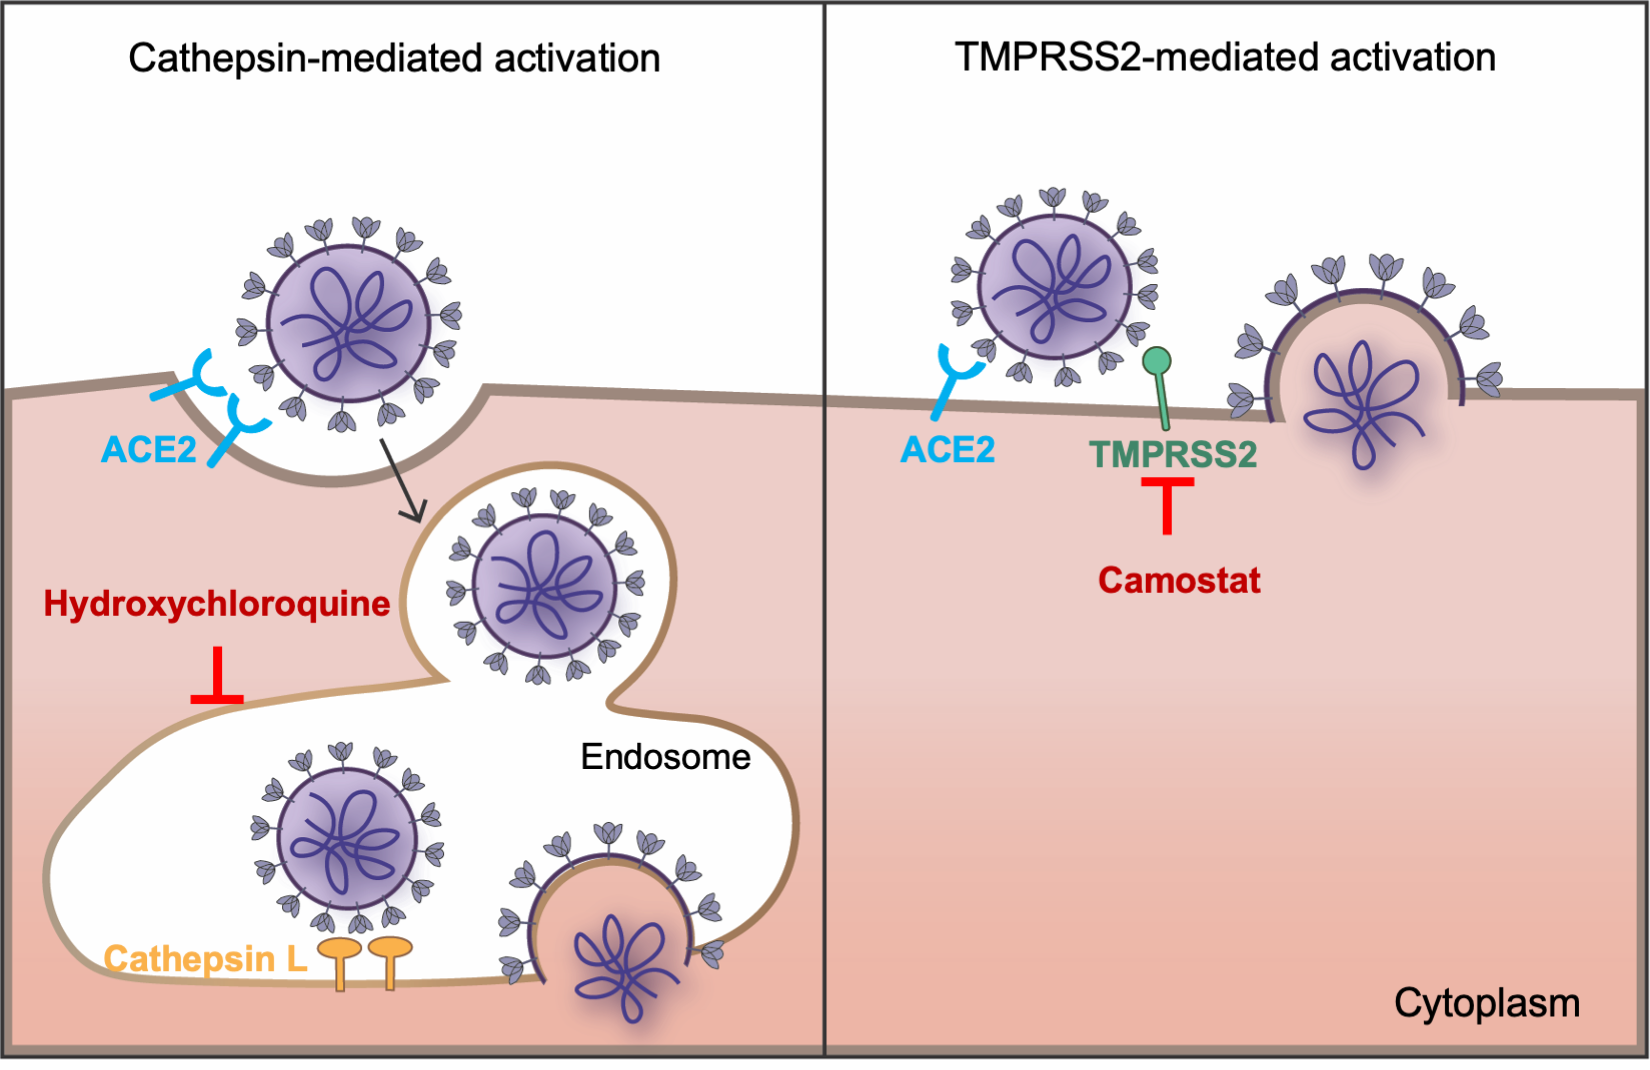
\includegraphics[scale=0.75, frame] {images/fusion.png}}
\caption{SARS-CoV-1 and SARS-CoV-2 fusion and cell entry can be activated by either or both of two pathways \cite{covid:cleavage}}
\label{fig:fusion}
\end{figure}

	
\item S2 bends around and brings the host cell membrane into contact
with the viral membrane. This is the post fusion state.
\end{enumerate}


\newpage
\bibliographystyle{plain}
\bibliography{/Users/dmm/papers/bib/biology}


\end{document} 

